%%%%%%%%%%%%%%%%%%%%%%%%%%%%%%%%%%%%%%%%%%%%%%%%%%%%%%%%%%%%%
%
% Exercises template
%
% Author: Francisco Luque Sánchez (@pacron on github)
%
% Feel free to download, use and share this template :)
%
%%%%%%%%%%%%%%%%%%%%%%%%%%%%%%%%%%%%%%%%%%%%%%%%%%%%%%%%%%%%

\documentclass[12pt]{article}       % class document and font size
\usepackage[utf8]{inputenc}       % allowance of accents (spanish writing)
\usepackage{graphicx}               % graphic package, for embedding images
\usepackage{listings}               % attach code to document
\usepackage{color}                  % define your own awesome colors

% some stuff for quality tables (english doc: http://osl.ugr.es/CTAN/macros/latex/contrib/booktabs/booktabs.pdf)
\usepackage{booktabs}
\usepackage{multirow}   
\usepackage{tikz}         
\usepackage{multicol}
\usepackage{hhline}

\usetikzlibrary{positioning,arrows}
% color definition for code listing
\definecolor{mygreen}{rgb}{0,0.6,0}
\definecolor{mygray}{rgb}{0.5,0.5,0.5}
\definecolor{mymauve}{rgb}{0.58,0,0.82}

% code listing settings; you can look for settings parameters here: (http://bfy.tw/2BN5)
\lstset{
  backgroundcolor=\color{white},   % choose the background color; you must add \usepackage{color} or \usepackage{xcolor}
  basicstyle=\scriptsize\ttfamily, % the size of the fonts that are used for the code
  breakatwhitespace=false,         % sets if automatic breaks should only happen at whitespace
  breaklines=true,                 % sets automatic line breaking
  captionpos=b,                    % sets the caption-position to bottom
  commentstyle=\color{mygreen},    % comment style
  deletekeywords={...},            % if you want to delete keywords from the given language
  escapeinside={\%*}{*)},          % if you want to add LaTeX within your code
  extendedchars=true,              % lets you use non-ASCII characters; for 8-bits encodings only, does not work with UTF-8
  frame=single,                    % adds a frame around the code
  keepspaces=true,                 % keeps spaces in text, useful for keeping indentation of code (possibly needs columns=flexible)
  keywordstyle=\color{blue},       % keyword style
  otherkeywords={*,...},           % if you want to add more keywords to the set
  numbers=left,                    % where to put the line-numbers; possible values are (none, left, right)
  numbersep=5pt,                   % how far the line-numbers are from the code
  numberstyle=\tiny\color{mygray}, % the style that is used for the line-numbers
  rulecolor=\color{black},         % if not set, the frame-color may be changed on line-breaks within not-black text (e.g. comments (green here))
  showspaces=false,                % show spaces everywhere adding particular underscores; it overrides 'showstringspaces'
  showstringspaces=false,          % underline spaces within strings only
  showtabs=false,                  % show tabs within strings adding particular underscores
  stepnumber=2,                    % the step between two line-numbers. If it's 1, each line will be numbered
  stringstyle=\color{mymauve},     % string literal style
  tabsize=2,                       % sets default tabsize to 2 spaces
  title=\lstname                   % show the filename of files included with \lstinputlisting; also try caption instead of title
}

% Change the tolerance of hyphenation tool
\pretolerance=2000
\tolerance=3000


\title{Practica 2 - Ejercicio 5\\
       \huge Protocolo de aplicación - Tchat}

% Own header
\author{
        María del Mar Ruiz Martín\\
        Francisco Luque Sánchez\\
        Doble Grado de Ingeniería Informática y Matemáticas\\
}
\date{\today}

\begin{document}
\maketitle

\section{Descripción de la aplicación}
En esta práctica se va a desarrollar e implementar un protocolo de aplicación. En nuestro caso, vamos a desarrollar un pequeño servicio de mensajería instantánea para la terminal de linux, Tchat, que tendrá dos funcionalidades básicas. Por un lado, permitirá conectarse con otros usuarios directamente, para tener una conversación entre dos personas. Por otro, permitirá crear salas de chat en las que pueden entrar varios usuarios e interactuar entre sí. Además, tendremos una pantalla principal en la que tendremos los usuarios que están conectados en ese momento, así como las salas de chat global abiertas.\\

Para realizar esta conexión, tendremos un servidor que controlará los usuarios que hay conectados a la red (usando un servicio de directorio), y que permitirá que unos usuarios se conecten a otros. Además, será el encargado de gestionar el funcionamiento de las salas de chat, recibiendo los mensajes y enviándoselos a todos los 
usuarios conectados a dicha sala de chat.\\

La conexión entre dos usuarios, en cambio, será individual, es decir, el servidor enviará a ambos la dirección del otro, y se establecerá una conexión entre ellos, sin que los mensajes tengan que pasar por el servidor.

\section{Diagrama de estados del servidor}

Veamos ahora el diagrama de estados del servidor:

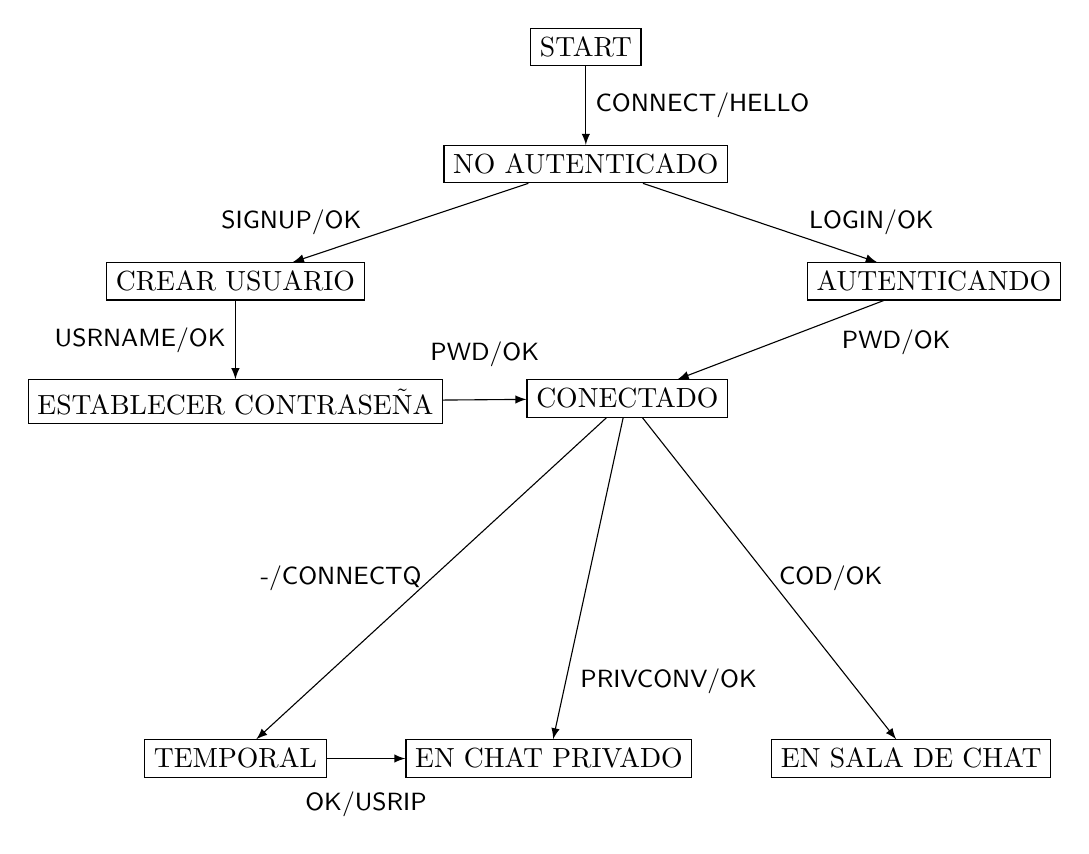
\begin{tikzpicture}
%% Nodes definition
\node[rectangle, draw] (start) {START};
\node[rectangle, draw, below = of start] (not_auth) {NO AUTENTICADO};
\node[rectangle, draw, below left = of not_auth] (create_usr) {CREAR USUARIO};
\node[rectangle, draw, below = of create_usr] (set_pwd) {ESTABLECER CONTRASEÑA};
\node[rectangle, draw, below right = of not_auth] (auth) {AUTENTICANDO};
\node[rectangle, draw, below left = of auth] (connected) {CONECTADO};
\node[rectangle, draw, below = 4cm of set_pwd] (temp) {TEMPORAL};
\node[rectangle, draw, right = of temp] (priv_chat) {EN CHAT PRIVADO};
\node[rectangle, draw, right = of priv_chat] (chat_room) {EN SALA DE CHAT};

%% Edges definition
\path[every node/.style={font=\sffamily\small}, every edge/.append style={>=latex}]
    (start) edge [->] node[right] {CONNECT/HELLO} (not_auth)
    (not_auth) edge [->] node[left=0.5cm] {SIGNUP/OK} (create_usr)
    (create_usr) edge [->] node[left] {USRNAME/OK} (set_pwd)
    (set_pwd) edge [->] node[above=0.3cm] {PWD/OK} (connected)
    (not_auth) edge [->] node[right=0.5cm] {LOGIN/OK} (auth)
    (auth) edge [->] node[below right, near start] {PWD/OK} (connected)
    (connected) edge [->] node[left] {-/CONNECTQ} (temp)
    (connected) edge [->] node[below right, near end] {PRIVCONV/OK} (priv_chat)
    (temp) edge [->] node[below=0.3cm] {OK/USRIP} (priv_chat)
    (connected) edge [->] node[right] {COD/OK} (chat_room)
    % (node4) edge [->] node[above] {a} (node5)
    % (node5) edge [->, bend right] node[below] {a} (node6)
    % (node5) edge [->] node[above] {b} (node7)
    % (node6) edge [->, bend right] node[below] {a} (node5)
    % (node6) edge [->] node[above] {b} (node7)
    % (node7) edge [->, loop right] node[right] {a,b} (node7)
    ;
\end{tikzpicture}


\end{document}